% !TeX root = ../main.tex
% Add the above to each chapter to make compiling the PDF easier in some editors.

\chapter{Approach}\label{chapter:Approach}
In this chapter, the proposed solution to tackling pervasive computing and data distribution of context-aware input sensor data is unfolded. At the beginning, a broad perspective of the architecture is demonstrated, followed by, the explanation of modeling input sensor data. Then, two sections describing pervasive computing and data distribution models and architectures. Finally, a description of the communication model is disclosed.
\section{System Design }
A System Design can be broadly described as an architecture of the system, which includes an explanation of each and every hardware component of the system, the connection between these components if there is any, and the data flowing between these components. Moreover, it provides a wide glimpse of the whole system but not its exact functionality, hence, giving a simple understanding of the architecture without jumping into much detail.\\
Initially, the components of the System Design is introduced, then, the connection between these components is shown, and eventually, the flow of the data is pointed out.

\subsection{Components}
\label{sub:components}
Below, each component of the proposed system design is explained.

\subsubsection{Node}
\label{subsub:node}
%The first set of components to explain are the sensors, they refer to objects that detect certain change in the environment and converts these changes into digital data and 
%which refer to objects that can detect certain changes in the environment and converts them to digital data, 
A Node is one of the core components of this design, it is a small computer device of low storage and computation capacity compared to nowadays portable computers, commonly a \textit{Raspberry Pi} but could be any other device. It is connected to several sensors which typically detect certain changes in the environment and converts it into digital data, for instance, Gas sensor, Temperature sensor or a Camera. Then, the device either stores the data into a local database, performs a computation locally, does both or even asks other nodes to do computation instead, however, an assumption about which sensors or specifications does a specific node  possess can not be made, meaning, each node might not have the exact number or types of sensors because each node may be deployed in a different timing or context. Thus, each node has a configuration file specifying its capabilities. A typical node is shown in figure \ref{fig:node}

\begin{figure}[H]
\centering
 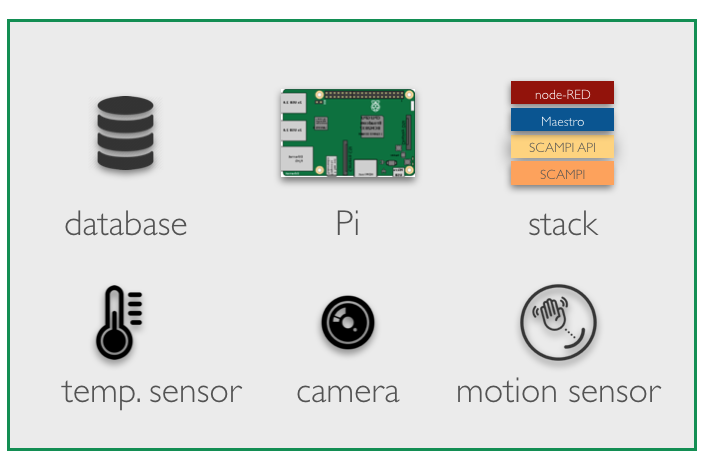
\includegraphics[scale=0.4]{images/node.png}
 \caption{A typical node in the system}
 \label{fig:node}
\end{figure}

\subsubsection{Graphics Processing Unit }

A Graphics Processing Unit \textit{GPU} is a device with massively parallel architecture designed to handle multiple tasks at the same time, thus observed to be much faster and more efficient than a Central Processing Unit \textit{CPU}, and in turn, has higher computation capabilities than the CPUs in the proposed system nodes in \ref{subsub:node}

\begin{figure}[H]
	\centering
	
\includegraphics[scale=0.7]{images/gpu.png}
		\caption{Figure denoting a Graphics Processing Unit GPU}
	\label{fig:gpu}
\end{figure}

\subsubsection{Network}
\label{subsub:network}
A Network in this design is a set of connected components which are capable of communicating and therefore allowing data sharing between them.
\begin{figure}[H]
	\centering
	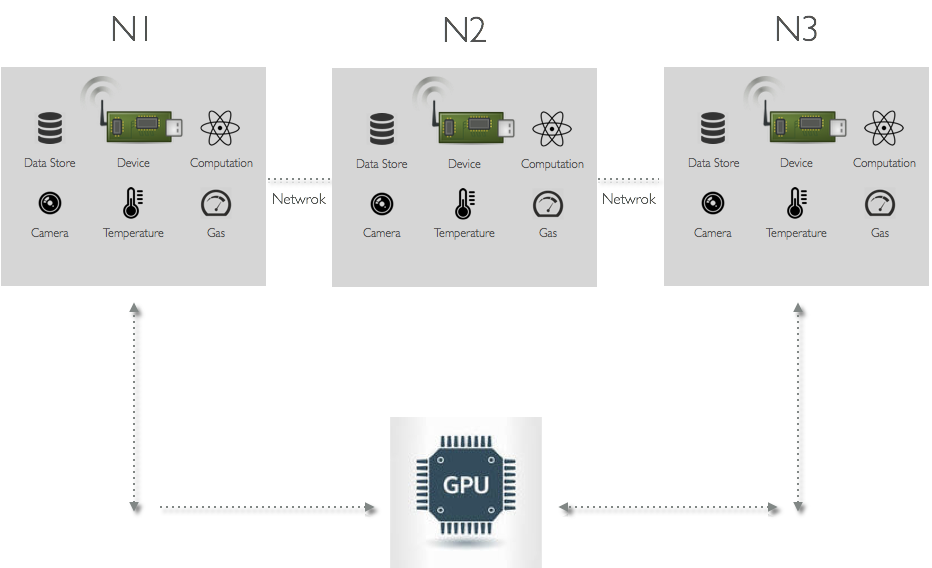
\includegraphics[scale=0.4]{images/network.png}
	\caption{A network consisting of three connected nodes and a GPU}
	\label{fig:network}
\end{figure}

\subsubsection{Mobile Device}
A Mobile Device in this context is any device that can connect to the network containing the nodes and is allowed to  carry data from one network to another, hence, allowing a form of data sharing between networks or nodes which are not connected.

\begin{figure}[H]
	\centering
	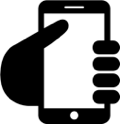
\includegraphics[scale=0.3]{images/mobile.png}
	\caption{Figure denoting a Mobile Device}
	\label{fig:mobile}
\end{figure}



\subsection{Connectivity and Data Flow}
A Network described in \ref{subsub:network}, is a simple form of connectivity between components, however, components and specifically nodes are not necessarily connected, sometimes they are just a standalone component that cannot share any information via direct connectivity, also, networks could be disconnected as well, meaning, a network might not be connected to the whole system, thus, is a standalone network. In these cases, a mobile device could help in carrying information and data between these disconnected nodes or networks. 

\begin{figure}[H]
	\centering
	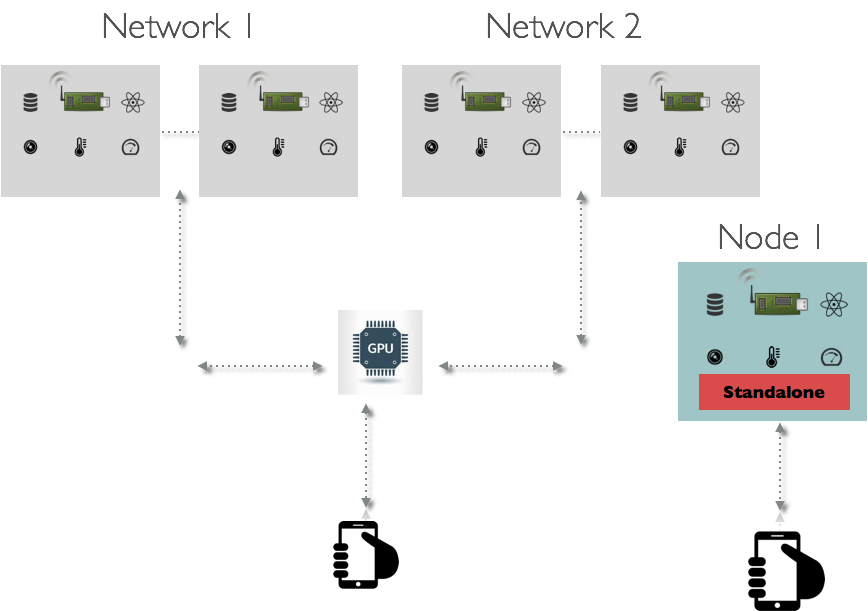
\includegraphics[scale=0.5]{images/system.png}
	\label{fig:system}
	\caption{Two networks connected with a GPU and one standalone network}
\end{figure}






\section{Modeling of Input Sensor Data}
\subsection{Show how the different sensors have data been modeled to fit our requirements for further use in computations}
\subsection{Dealing with Resources}
\subsubsection{We cant make assumptions about resources}
\subsubsection{Resource capability description " Resource Configuration File"}
\subsubsection{Decoupling Resources}



\section{Pushing the Computation to the Edges "Nodes"}

\subsection{Execution Model}
- Which nodes should execute the data, is it all, some  or a specific nodes. Also, how is the model specified in the computation meta data.
- How do we know if a Computational Instance has been executed or not.

\newpage
\subsubsection{Computation Meta-Model}
Since the goal is to push computations to the available nodes which have the capability to do so, there are three main aspects that must be addressed to achieve this goal.
\begin{itemize}
	
\item First, is to be able to express the computational requirements and resources that the computation is going to use while running on a specific node, which is also called \textbf{"Compuation Meta-data"}. Since we cannot make assumptions that a certain node has specific resources or specification as explained in \ref{subsub:node}, these requirements has to be pushed along with the computation. It includes, for instance, the amount of processing power and random access memory the computation is going to need, also, the resources required to perform such a computation.
The meta-data is expressed as a \textit{JSON} formatted object.

\textbf{include example}

\item Second, is the core of the meta-model, which is a model expressing the computation itself, and since node-red is the chosen platform to execute our computation on, then naturally, it is modeled into a \textit{flow}, which is a model used by node-red to describe the capabilities and actions of a computation in JSON format. This simplifies the whole idea of making the computation meta-model travel through the network, because with node-red, the maintainer could develop a computation using the user interface of node-red, then export this computation as a flow, include the meta-data and publish it to the network. Afterwards, a node can read the meta-data and analyze if it could run this computation according to its resources, then import the flow into its node-red instance and deploy it for running.
\textbf{include example}

\item Last aspect in the meta-model is the output or results of the computation run. Since the node does not know what kind of data does the computation produce, therefore the maintainer must specify the way the output data is used or stored. In this case, nodes can understand whether the data needs to be sent back to the original node or just stored in a local database for further use. \\
\textbf{include example}
\end{itemize}
\subsubsection{Dealing with Dependencies ( Shipping, Configuring)}


\section{Moving Data}
\subsection{Explain data distribution among several nodes to apply pervasive computing}

\subsubsection{Input Meta-data}
is it local, provided or collected data.
% moreover, the way that the input data used while doing this computation will be provided, whether it gets the input data from a local database or is it going to be included along with the computational data. 

\section{Networking}
\subsection{SCAMPI }







